
    
\documentclass[12pt]{article}

\usepackage[margin=1in]{geometry}

% For using float option H that places figures exatcly where we want them
\usepackage{float}
% makes figure font bold
\usepackage{caption}
\captionsetup[figure]{labelfont=bf}
% For text generation
\usepackage{lipsum}
% For drawing
\usepackage{tikz}
% For smaller or equal sign and not divide sign
\usepackage{amssymb}
% For the diagonal fraction
\usepackage{xfrac}
% For enumerating exercise parts with letters instead of numbers
\usepackage{enumitem}
% For dfrac, which forces the fraction to be in display mode (large) e
% even in math mode (small)
\usepackage{amsmath}
% For degree sign
\usepackage{gensymb}
% For "\mathbb" macro
\usepackage{amsfonts}
\newcommand{\N}{\mathbb{N}}
\newcommand{\Z}{\mathbb{Z}}
\newcommand{\Q}{\mathbb{Q}}
\newcommand{\R}{\mathbb{R}}
\newcommand{\C}{\mathbb{C}}

% overline short italic
\newcommand{\olsi}[1]{\,\overline{\!{#1}}}

\usepackage{indentfirst}
\usetikzlibrary{shapes,positioning,fit,calc}

\usepackage{changepage} % for adjustwidth environment

\title{%
    \Huge Abstract Algebra \\
    \large by \\
    \Large Dummit and Foote \\~\\
    \huge Part 1: Group Theory \\
    \LARGE Chapter 1: Introduction to Groups \\
    \Large Section 2: Dihedral Groups
}
\date{2024-03-06}
\author{Michael Saba}

\begin{document}
    \pagenumbering{gobble}
    \maketitle
    \newpage
    \pagenumbering{arabic}


    An important family of groups
    is the family of Dihedral groups,
    where each group is comprised corresponds to the set of symmetries 
    that can be performed on a geometric object
    while keeping its shape intact. \\

    \subsection*{Dihedral Groups}

    \textbf{Dihedral groups} are the family of groups
    made up of the rigid motions that can be performed on regular polygons
    in $\R^3$ ($3$D space)
    while keeping the shape of the polygon intact,
    such that it can be placed back over the original
    and perfectly cover it.
    The motions have to be rigid,
    in the sense that the polygons can only be moved around in $R^3$
    before being placed back over the original shape. \\
    More formally,
    each symmetry in a dihedral group must permute the vertices of a polygon
    while keeping the relative positions of the vertices intact as to
    not deform it.
    The permuation here maps each vertex from the original shape
    to the vertex it comes to cover afer the symmetry has been performed. \\

    Each group is denoted $D_{2n}$,
    where $n$ is the number of vertices the polygon in question has.
    Most books on groups theory use the the $D_n$ notation,
    but this book does not. \\

    Examples of symmetries that can be perfomed
    while keeping a polygon intact include rotation by some angle,
    and reflection
    (which counts as a rigid motion as reflecting a $2$D polygon
    is the same as flipping it in $\R^3$ space around an axis). \\ 
    Notice how in the images,
    the location of the vertices is permuted,
    but the shape of the square remains the same,
    and the position of the vertices relative to each other is the same.
    For instance, there can never be a rigid motion that places
    $A$ and $C$ adjacently,
    as that deforms the square. \\

    \begin{figure}[H]
        \centering
        \begin{tikzpicture}
            \def\side{2} % Define the distance between vertices
            \coordinate (A1) at (0, 0);
            \coordinate (A2) at (\side, 0);
            \coordinate (A3) at (\side, \side);
            \coordinate (A4) at (0, \side);

            \node at (A1)[below left] {$A$};
            \node at (A2)[below right] {$B$};                
            \node at (A3)[above right] {$C$};    
            \node at (A4)[above left] {$D$};  
            
            \draw (A1) -- (A2) -- (A3) -- (A4) -- cycle;

            \foreach \i in {1, 2, 3, 4}
            \coordinate (B\i) at ($(A\i) + (6, 0)$);

            \node at (B1)[below left] {$D$};
            \node at (B2)[below right] {$A$};                
            \node at (B3)[above right] {$B$};    
            \node at (B4)[above left] {$C$};  
            
            \draw (B1) -- (B2) -- (B3) -- (B4) -- cycle;
            \draw[->] (3 , 1) -- (5, 1);
            \node at (4, 1)[above, font=\small, align=center]
            {Rotation \\ by $90\degree$};

        \end{tikzpicture}  
        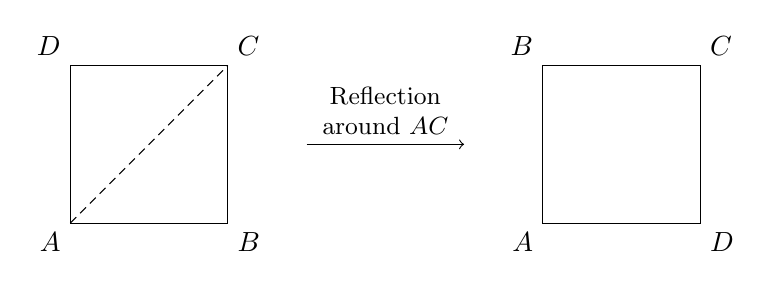
\begin{tikzpicture}
            \def\side{2} % Define the distance between vertices
            \coordinate (A1) at (0, 0);
            \coordinate (A2) at (\side, 0);
            \coordinate (A3) at (\side, \side);
            \coordinate (A4) at (0, \side);

            \node at (A1)[below left] {$A$};
            \node at (A2)[below right] {$B$};                
            \node at (A3)[above right] {$C$};    
            \node at (A4)[above left] {$D$};  
            
            \draw (A1) -- (A2) -- (A3) -- (A4) -- cycle;

            \foreach \i in {1, 2, 3, 4}
            \coordinate (B\i) at ($(A\i) + (6, 0)$);

            \node at (B1)[below left] {$A$};
            \node at (B2)[below right] {$D$};                
            \node at (B3)[above right] {$C$};    
            \node at (B4)[above left] {$B$};  
            
            \draw (B1) -- (B2) -- (B3) -- (B4) -- cycle;
            \draw [densely dashed] (A1) -- (A3);

            \draw[->] (3 , 1) -- (5, 1);
            \node at (4, 1)[above, font=\small, align=center]
            {Reflection \\ around $AC$};
        \end{tikzpicture}  

        \caption{\label{fig:figure1} Symmetries applied on a square.}
    \end{figure}

    To denote a rigid motion in a dihedral group,
    we use $\sigma$.
    Recall that in $D_{2n}$,
    $\sigma$ is no more than a permutation
    of the vertices $\{1, 2, 3 \dots n\}$. \\
    Not all permutations of the set are elements of the $D_{2n}$ however,
    only those that map the elements onto other elements in such a way
    as to preserve the relative distances of the polygon.
    The permutation simply describes where each vertex ends up on the
    original polygon after having performed a rigid motion. \\

    Permutations of $S = \{1, 2, 3 \dots n\}$ are just functions
    $f: S \rightarrow S$ that map each element in $S$ to exactly
    one other in $S$.
    Since all elements of dihedral groups are permuations,
    and by extension, functions,
    this means that the group operator of dihedral groups
    is function composition $\circ$.
    If we have two elements of $D_{2n}$, $\sigma: S \rightarrow S$
    and $\tau: S \rightarrow S$,
    then $\sigma \circ \tau$
    is the composition of the two, read from right to left. \\
    So a vertex $k$ transformed by $\sigma \circ \tau$
    is first permuted by $\tau$,
    then the resulting vertex $\tau(k)$ is permuted by $\sigma$
    to give a result of $\sigma(\tau(k))$. \\
    Note that because groups are closed under their operators,
    the resulting permuation is also necessarily a rigid motion. \\

    The identity of any dihedral group is the transformation
    that leaves all the vertices in place (the motion that does nothing).
    We denote it using 1 and call it the identity symmetry. \\

    The inverse of any transformation in a dihedral group
    is the reverse transformation;
    the one that returns the vertices to their original location. \\

    The order of any dihedral group $D_{2n}$ is $2n$.
    We can show that this is the case with a simple proof. \\
    Suppose we hav an arbitrary n-gon with vertices $\{1, 2 \dots n\}$.
    \begin{figure}[H]
        \centering
        \begin{tikzpicture}
            \def\side{2} % Define the distance between vertices
            \coordinate (A1) at (0, 0);
            \coordinate (A2) at (\side, 0);
            \coordinate (A4) at (0, \side);
            \coordinate (A5) at (\side + 1, 1);
            \coordinate (A6) at (1, \side + 1);

            \node at (A1)[below left] {$1$};
            \node at (A2)[below right] {$2$};                   
            \node at (A4)[above left] {$n$};  
            
            \draw (A2) -- (A1) -- (A4);
            \draw[densely dashed] (A2) -- (A5);
            \draw[densely dashed] (A4) -- (A6);

        \end{tikzpicture}  
        \caption{\label{fig:figure1} Symmetries applied on a square.}
    \end{figure}
    \noindent We recall that the transformation has to move
    the vertices to other vertices in the polygon while keeping
    the relative positions intact. \\
    So we start with vertex $1$.
    We can conceivably move it to any other vertex in the polygon,
    without necessarily deforming the shape. 
    This gives us $n$ possible mappings. \\
    At this point, we know that the vertex $2$
    has to be next to vertex $1$.
    However, we can conceive that the vertex will end up
    on either side of $1$,
    the left or right side. \\
    Sure, depending on the side that $2$ is on,
    the order of the vertices may go from counter-clockwise to clockwise,
    but since vertex $2$ is still next to first vertex,
    no deforming has been done. \\
    At the point, vertex $3$ is fixed;
    we already know it had to be next to vertex $2$,
    and since vertex $1$ occupies one of the sides,
    its position is already determined.
    The same applies for all other vertices. \\
    In other words, the position of vertices $1$ and $2$
    determine the entire transformation.
    With that said, there must be $2 \times n$ transformations,
    as there are $n$ positions on which to place vertex $1$
    and then positions on which we can then place vertex $2$. \\  
    We thus conclude that $|D_{2n}| = 2n$. \\

    We can explicitely define these $2n$ transformations. \\
    First, we can obviously rotate the polygons
    around their center $n$ times,
    each time shifting the vertices by $1$
    such that vertex $k$ ends up at $(k + 1)\mod n$.
    Starting with $k = 0$ for the identity symmetry,
    the angle of the $k^{\text{th}}$ rotation
    is $\sfrac{2\pi k}{n}$ radian. \\
    The other $n$ transformations are all reflections.
    When $n$ is odd,
    then each axis of symmetry around which we reflect the polygon
    will pass through a unique vertex,
    and the middle of the opposing edge.
    When $n$ is even,
    then half of the axes will connect opposing vertices,
    and the other half will connect opposing edges at their mid-points. \\
    Of course, we still need to show that the transformations
    we described are unique
    (for example that no rotation is equivalent to a reflection). \\
    \begin{figure}[H]
        \centering
        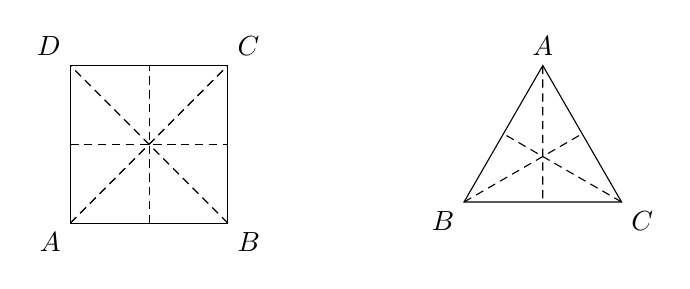
\begin{tikzpicture}
            \def\side{2} % Define the distance between vertices
            \coordinate (A1) at (0, 0);
            \coordinate (A2) at (\side, 0);
            \coordinate (A3) at (\side, \side);
            \coordinate (A4) at (0, \side);

            \node at (A1)[below left] {$A$};
            \node at (A2)[below right] {$B$};                
            \node at (A3)[above right] {$C$};    
            \node at (A4)[above left] {$D$};  
            
            \draw (A1) -- (A2) -- (A3) -- (A4) -- cycle;

            \def\height{\side*sqrt(3)/2} % Define the distance between vertices
            \coordinate (B1) at (6, 2);
            \coordinate (B2) at ({6 - \side/2}, {2-\height});
            \coordinate (B3) at ({6 + \side/2}, {2-\height});


            \node at (B1)[above] {$A$};
            \node at (B2)[below left] {$B$};                
            \node at (B3)[below right] {$C$};     
            
            \draw (B1) -- (B2) -- (B3) -- cycle;
            \draw [densely dashed] (A1) -- (A3);
            \draw [densely dashed] (A2) -- (A4);
            \draw [densely dashed] (A1) -- (A3);
            \draw [densely dashed] (0, 1) -- (2, 1);
            \draw [densely dashed] (1, 0) -- (1, 2);
            \coordinate (M12) at ($(B1)!.5!(B2)$);
            \coordinate (M23) at ($(B2)!.5!(B3)$);
            \coordinate (M31) at ($(B3)!.5!(B1)$);
            \draw[densely dashed] (B1) -- (M23);
            \draw[densely dashed] (B2) -- (M31);
            \draw[densely dashed] (B3) -- (M12);

        \end{tikzpicture}  

        \caption{\label{fig:figure1} Symmetry axes
        of a polygons with an even and odd number of vertices.}
    \end{figure}

    Later on, we will see that we only need a single reflection,
    and that we can express the rest as rotations of the shape
    after it has been reflected (we can also rotate then reflect). 
    The one reflection that we will need is the one around the axis
    that connects vertex $1$ to the centroid of the polygon.
    (we can use any reflection, but by convention,
    this one is used to simplify calculations). 
    Depending on wether $n$ is odd or even,
    this axis may connect the first vertex to an ooposite vertex,
    or an opposite edge.
    We call this reflection $s$. \\ 
    Likewise, we can usually express rotations in terms of the 
    first rotation, by an angle of $\sfrac{2\pi}{n}$.
    For instance, a rotation $\sfrac{4\pi}{n}$
    is just two repeated rotations of angle $\sfrac{2\pi}{n}$.
    We will call this rotation $r$. \\

    We can now derive some basic properties:
    \begin{itemize}[label=$\diamond$]
        \item 
            The elements $r^0, r^1 \dots r^{n-1}$ are all distinct.
            Moreover $r^0 = 1$ (no rotation),
            and $r^n = 1$ (rotation by $2\pi$).
            That means that necessarily, $|r| = n$
            (the smallest power to which $r = 1$).
        \item 
            Reflecting twice $s^2$ is the same as doing nothing,
            so $|s| = 2$
            (since $s \neq 1$,
            making $2$ the smallest power for which the property holds).
        \item
            We have that $s \neq r^i$ for any $i$.
            This is because rotations keep the order of the vertices intact,
            while reflections transform them from
            counter-clockwise to clockwise,
            so the vertices have to end up in different positions.
        \item
            We know that $sr^{i} \neq sr^j$
            for any $0 \leqslant i, j \leqslant n-1$ where $i \neq j$.
            This follows from the first point.
            Furthermore, this tells us that all elements can be written
            in the form of $r^i$ or $sr^i$
            where $0 \leqslant i \leqslant n-1$.
            Note that since rotations account for $n$ elements
            (all those of the form $r^i$)
            it must be that the $n$ reflections
            correspond to the remaining elements of the form $sr^i$.
            So all reflections can be expressed in terms of a single reflection.
            This makes sense, since all reflections share the action
            of transforming the order of the vertices 
            from counter-clockwise to clockwise and vice-versa,
            the only thing that differs between them is the angle
            of the axis along which the reflection is made,
            meaning any axis's reflection can be replicated by
            simply rotating the object first
            (since composition is read right to left,
            $r^i$ is done first in $sr^i$). \\
            This also tells us that the multiplication of any
            elements of the form $s^kr^i$
            will produce an element of the same form.
        \item
            We have $rs = sr^{-1}$.
            As $s$ and $r$ don't compute,
            this proves $D_{2n}$ is never abelian.
            We can prove this statement by examining what each permutation
            does to an $n$-gon.
            The former reflects it then rotates it
            (read from right to left).
            The latter does the rotation $r^{-1}$
            (rotates by the same angle as $r$ but to the other side,
            since it's supposed to reverse the action of $r$)
            then reflects it.
            We can visually see that they are the same.
            This makes sense;
            because reflecting switches the order of the vertices,
            a rotation counter-clockwise side becomes the same rotation,
            but clockwise. \\

            \begin{figure}[H]
                \centering 
                \begin{tikzpicture}
                    \def\side{2} % Define the distance between vertices
                    \coordinate (A1) at (0, 0);
                    \coordinate (A2) at (\side, 0);
                    \coordinate (A3) at (\side, \side);
                    \coordinate (A4) at (0, \side);
        
                    \node at (A1)[below left] {$1$};
                    \node at (A2)[below right] {$2$};                  
                    \node at (A4)[above left] {$n$};  
                    
                    \draw (A2) -- (A1) -- (A4);
        
                    \foreach \i in {1, 2, 3, 4}
                    \coordinate (B\i) at ($(A\i) + (6, 0)$);
        
                    \node at (B1)[below left] {$1$};
                    \node at (B2)[below right] {$n$};                   
                    \node at (B4)[above left] {$2$};  
                    
                    \draw (B2) -- (B1) -- (B4);
                    \draw [densely dashed] (A1) -- (A3);
        
                    \draw[->] (3 , 1) -- (5, 1);
                    \node at (4, 1)[above, font=\small, align=center]
                    {Reflection $s$};

                    \foreach \i in {1, 2, 4}
                    \coordinate (C\i) at ($(B\i) + (6, 0)$);
        
                    \node at (C1)[below left] {$2$};
                    \node at (C2)[below right] {$1$};                   
                    \node at (C4)[above left] {$3$};  
                    
                    \draw (C2) -- (C1) -- (C4);
        
                    \draw[->] (9 , 1) -- (11, 1);
                    \draw[->] (7.1,1.4) arc (90:360:0.4);
                    \node at (10, 1)[above, font=\small, align=center]
                    {Rotation $r$};
                \end{tikzpicture}  
        
                \caption{\label{fig:figure1}
                Transformation of $rs$.}
            \end{figure}    
            \begin{figure}[H]
                \centering 
                \begin{tikzpicture}
                    \def\side{2} % Define the distance between vertices
                    \coordinate (A1) at (0, 0);
                    \coordinate (A2) at (\side, 0);
                    \coordinate (A3) at (\side, \side);
                    \coordinate (A4) at (0, \side);
        
                    \node at (A1)[below left] {$1$};
                    \node at (A2)[below right] {$2$};                  
                    \node at (A4)[above left] {$n$};  
                    
                    \draw (A2) -- (A1) -- (A4);
        
                    \foreach \i in {1, 2, 3, 4}
                    \coordinate (B\i) at ($(A\i) + (6, 0)$);
        
                    \node at (B1)[below left] {$1$};
                    \node at (B2)[below right] {$3$};                   
                    \node at (B4)[above left] {$2$};  
                    
                    \draw (B2) -- (B1) -- (B4);
                    \draw [densely dashed] (B1) -- (B3);
        
                    \draw[->] (3 , 1) -- (5, 1);
                    \node at (4, 1)[above, font=\small, align=center]
                    {Rotation $r^{-1}$};

                    \foreach \i in {1, 2, 4}
                    \coordinate (C\i) at ($(B\i) + (6, 0)$);
        
                    \node at (C1)[below left] {$1$};
                    \node at (C2)[below right] {$2$};                   
                    \node at (C4)[above left] {$3$};  
                    
                    \draw (C2) -- (C1) -- (C4);
        
                    \draw[->] (9 , 1) -- (11, 1);
                    \draw[<-] (1.1, 1.4) arc (90:360:0.4);
                    \node at (10, 1)[above, font=\small, align=center]
                    {Reflection $s$};
                \end{tikzpicture}  
        
                \caption{\label{fig:figure1}
                Transformation of $rs$.}
            \end{figure}       
        
        \item
            We can extend the property so that $r^is = sr^{-i}$
            for $0 \leqslant i \leqslant n-1$.
            We can prove it using induction. \\
            \begin{adjustwidth}{1cm}{1cm}
                \textbf{Basis step:}
                We know that for $n = 1$,
                $rs = sr^{-1}$. \\
                \textbf{Inductive hypothesis:}
                Assume that for $n = k$,
                $r^ks = sr^{-k}$. \\
                \textbf{Inductive step:}
                Based on our assumptions,
                we know that $r^ks = sr^{-k}$.
                Now, let's multiply both sides by $r$.
                We get $rr^ks = rsr^{-k}$,
                which is $r^{k+1}s = (rs)r^{-k}$.
                We also know that $r^ks = sr^{-k}$,
                so we can modify the right hand side such that
                $r^{k+1}s = (sr^{-1})r^{-k} = sr^{-1}r^{-k} = sr^{-k-1}$.
            \end{adjustwidth}
            With that the proof is complete. \\
    \end{itemize}


    \subsection*{Generators and Relations}

    In $D_2n$, we can very simply represent any element
    using only two elements $r$ and $s$
    (each can be used more than once).
    We can generalize this idea for arbitrary groups.
    They will provide us with a simple and easy way of describing
    and computing in many groups.
    We won't rigorously describe them now,
    but we will introduce them so they be taken advantage of. \\

    If a groups $G$ has a subset $S$
    such that all elements of $G$ can be written as a finite
    product of the elements of $S$ and their inverses.
    (meaning that elements in $S$ can be raised to any finite power),
    we call $S$ a set of \textbf{generators} of $G$. \\
    We will indicate that $S$ generates $G$ using
    the $G = \langle S \rangle$ notation.
    If $S = \{a, b, c \dots\}$,
    we can also directly write $G = \langle a, b, c \dots \rangle$. \\
    To give an example of a group that can be generated by a subset,
    take the additive group of integers $\Z$,
    which can be generated using just $1$ (and its inverse $-1$),
    as all integers are just additions of $1$.
    So $\Z = \langle 1 \rangle$. \\
    Likewise, from our calculations,
    we can conclude that for any $n$, $D_{2n} = \langle r, s \rangle$. \\

    This is not mentioned in this part of the book but,
    note that a generating subset $S$ of $G$ doesn't need to be minimal
    (e.g. it may be able to generate all other elements without some of
    its element). \\
    If for any $x \in S$, $S - \{x\}$ can't generate $G$,
    then $S$ is a \textbf{minimal generating set}.
    This doesn't necessarily mean $S$ is the smallest set of generators
    of $G$,
    just that all the elements in $S$ are necessary
    in order to generate $G$. \\
    
    Although this will not yet be proven,
    it will later be shown that $S$ generates $G$
    if each element of $G$
    can be written as a finitie product of elements in $S$,
    not including the inverses. \\
    This is already clear in the case of $D_{2n}$,
    as all elements are of the form $r^i$ or $sr^{i}$
    for $0 \leqslant i \leqslant n-1$. \\

    Any equation in $G$ that can be satisfied by generators,
    such as $rs = sr^{-1}$ in $D_{2n}$,
    is called a \textbf{relation}. \\
    Sometimes, a set of relations also has the property that 
    any other relation between elements of the group can be derived
    using only its relations.
    For $D_{2n}$, the minimal number of relations that satisfies
    this property is three:
    $r^n = 1$, $s^2 = 1$, and $rs = sr^{-1}$. \\
    Note that we can use the identity $1$ even though it's not a generator;
    its the only element that doesn't need to be generated,
    as it's pretty much equal to $aa^{-1}$ for any element $a$. \\

    If a group $G$ is generated by $S$,
    and if there is a collection of relations $R_1, R_2 \dots R_m$
    (equations using products of elements in $S \cap \{1\}$)
    such that any other relation in the group can be derived
    from this collection, 
    then we will call these generators and relations
    a \textbf{presentation} of $G$,
    and it's denoted by
    \[ G = \langle S \mid R_1, R_2 \dots R_n \rangle \]
    For example,
    \[ D_{2n} = \langle r, s \mid r^n = s^2 = 1, rs = sr^{-1} \rangle \]
    Note that a group can have more than one presentation,
    since $G$ can have more than one set of generators,
    which in turn can be minimal or not.
    Same for relations.
    However, it is usually better to choose compact presentations,
    and only include necessary elements and relations. \\

    Using a presentation to represent a group can be far more
    concise than using a multiplication table,
    while carrying the same amount of information about the group. \\
    However, presentations have some limitations.
    It can sometimes be hard to tell if two elements expressed
    in terms of generators are the same or not using relations.
    This means that the order of a group isn't always evident
    from its presentation.
    For instance,
    \[ \langle x_1, y_1 \mid {x_1}^2 = {y_1}^2 = (x_1x_2)^2 = 1 \rangle \]
    is the presentation of a group of order $4$,
    and
    \[ \langle x_2, y_2 \mid {x_2}^3 = {y_2}^3 = (x_2x_2)^3 = 1 \rangle \]
    is the presentation of an infinite group. \\
    
    Another issue that occurs when using presentations 
    is called \textbf{collapsing}.
    This is when relations are intertwined in some unobvious way,
    such as having a hidden, implicit relation,
    that can be derived from the presentation but is not present in it. \\
    This makes it difficult to determine even a lower bound
    for the order of a group. \\
    Suppose we have 
    \[ X_{2n} = \langle x, y \mid x^n = y^2 = 1, xy = yx^2 \rangle \]
    This presentation seems similat to that of $D_{2n}$.
    It contains a commutation relation of its own, 
    which describes how to move x to the right of $y$,
    meaning that we should be able to represent any element 
    in the group as $y^kx^{m}$. \\
    We may assume this family of groups, like $D_{2n}$,
    have an order of $2n$,
    However, a hidden realtion:
    \[ x = xy^2 = (xy)y  = (yx^2)y = (yx)(xy) = (yx)(yx^2)
    = y(xy)x^2 = y(yx^2)x^2 = y^2x^4 = x^4 \]
    Since $x = x^4$,
    we can multiply both sides by the inverse and get that $x^3 = 3$.
    So $|x| \leqslant 3$,
    and, 
    since $|y| = 2$,
    this means that the group has at most order $6$. \\

    The reason we did not experience collapsing with $D_{2n}$
    is that we showed that $|D_{2n}| = 2n$
    by independent geometric means. \\


\end{document}
